%% BioMed_Central_Tex_Template_v1.06
%%                                      %
%  bmc_article.tex            ver: 1.06 %
%                                       %

%%IMPORTANT: do not delete the first line of this template
%%It must be present to enable the BMC Submission system to
%%recognise this template!!

%%%%%%%%%%%%%%%%%%%%%%%%%%%%%%%%%%%%%%%%%
%%                                     %%
%%  LaTeX template for BioMed Central  %%
%%     journal article submissions     %%
%%                                     %%
%%          <8 June 2012>              %%
%%                                     %%
%%                                     %%
%%%%%%%%%%%%%%%%%%%%%%%%%%%%%%%%%%%%%%%%%


%%%%%%%%%%%%%%%%%%%%%%%%%%%%%%%%%%%%%%%%%%%%%%%%%%%%%%%%%%%%%%%%%%%%%
%%                                                                 %%
%% For instructions on how to fill out this Tex template           %%
%% document please refer to Readme.html and the instructions for   %%
%% authors page on the biomed central website                      %%
%% http://www.biomedcentral.com/info/authors/                      %%
%%                                                                 %%
%% Please do not use \input{...} to include other tex files.       %%
%% Submit your LaTeX manuscript as one .tex document.              %%
%%                                                                 %%
%% All additional figures and files should be attached             %%
%% separately and not embedded in the \TeX\ document itself.       %%
%%                                                                 %%
%% BioMed Central currently use the MikTex distribution of         %%
%% TeX for Windows) of TeX and LaTeX.  This is available from      %%
%% http://www.miktex.org                                           %%
%%                                                                 %%
%%%%%%%%%%%%%%%%%%%%%%%%%%%%%%%%%%%%%%%%%%%%%%%%%%%%%%%%%%%%%%%%%%%%%

%%% additional documentclass options:
%  [doublespacing]
%  [linenumbers]   - put the line numbers on margins

%%% loading packages, author definitions

%\documentclass[twocolumn]{bmcart}
% uncomment this for twocolumn layout and comment line below
\documentclass{bmcart}

%%% Load packages
%\usepackage{amsthm,amsmath}
%\RequirePackage{natbib}
%\RequirePackage{hyperref}
\usepackage[utf8]{inputenc} %unicode support
\usepackage{graphicx}
\usepackage{tikz}
\usepackage{doi}
\usepackage{amsmath}
\usepackage{listings}
\usepackage{bera}
\usepackage{multirow}
%\usepackage[applemac]{inputenc} %applemac support if unicode package fails
%\usepackage[latin1]{inputenc} %UNIX support if unicode package fails
\lstdefinelanguage{json}{
    basicstyle=\normalfont\ttfamily,
    numbersep=8pt,
    showstringspaces=false,
    breaklines=true,
    frame=lines,
    backgroundcolor=\color{white},
}

%%%%%%%%%%%%%%%%%%%%%%%%%%%%%%%%%%%%%%%%%%%%%%%%%
%%                                             %%
%%  If you wish to display your graphics for   %%
%%  your own use using includegraphic or       %%
%%  includegraphics, then comment out the      %%
%%  following two lines of code.               %%
%%  NB: These line *must* be included when     %%
%%  submitting to BMC.                         %%
%%  All figure files must be submitted as      %%
%%  separate graphics through the BMC          %%
%%  submission process, not included in the    %%
%%  submitted article.                         %%
%%                                             %%
%%%%%%%%%%%%%%%%%%%%%%%%%%%%%%%%%%%%%%%%%%%%%%%%%


%\def\includegraphic{}
%\def\includegraphics{}



%%% Put your definitions there:
\startlocaldefs
\endlocaldefs


%%% Begin ...
\begin{document}

%%% Start of article front matter
\begin{frontmatter}

\begin{fmbox}
\dochead{Software}

%%%%%%%%%%%%%%%%%%%%%%%%%%%%%%%%%%%%%%%%%%%%%%
%%                                          %%
%% Enter the title of your article here     %%
%%                                          %%
%%%%%%%%%%%%%%%%%%%%%%%%%%%%%%%%%%%%%%%%%%%%%%

\title{gnparser: a Powerful Scientific Names Parser}

%%%%%%%%%%%%%%%%%%%%%%%%%%%%%%%%%%%%%%%%%%%%%%
%%                                          %%
%% Enter the authors here                   %%
%%                                          %%
%% Specify information, if available,       %%
%% in the form:                             %%
%%   <key>={<id1>,<id2>}                    %%
%%   <key>=                                 %%
%% Comment or delete the keys which are     %%
%% not used. Repeat \author command as much %%
%% as required.                             %%
%%                                          %%
%%%%%%%%%%%%%%%%%%%%%%%%%%%%%%%%%%%%%%%%%%%%%%

\author[
   addressref={aff1},
   corref={aff1},                       % id of corresponding address, if any
   email={dmozzherin@illinois.edu}
]{\inits{DYM}\fnm{Dmitry Y.} \snm{Mozzherin}}
\author[                  % id's of addresses, e.g. {aff1,aff2}
   noteref={n1},% id's of article notes, if any
   email={alexander.myltsev@phystech.edu}   % email address
]{\inits{AAM}\fnm{Alexander A.} \snm{Myltsev}}
\author[
   email={dpatterson.mbl@gmail.com}
]{\inits{DJP}\fnm{David J.} \snm{Patterson}}

%%%%%%%%%%%%%%%%%%%%%%%%%%%%%%%%%%%%%%%%%%%%%%
%%                                          %%
%% Enter the authors' addresses here        %%
%%                                          %%
%% Repeat \address commands as much as      %%
%% required.                                %%
%%                                          %%
%%%%%%%%%%%%%%%%%%%%%%%%%%%%%%%%%%%%%%%%%%%%%%

\address[id=aff1]{%                    % unique id
  \orgname{University of Illinois},    % university, etc
  \street{1816 South Oak St.},         %
  \city{Champaign},                    % city
  \state{IL},
  \postcode{61820},
  \cny{US}                             % country
}

%%%%%%%%%%%%%%%%%%%%%%%%%%%%%%%%%%%%%%%%%%%%%%
%%                                          %%
%% Enter short notes here                   %%
%%                                          %%
%% Short notes will be after addresses      %%
%% on first page.                           %%
%%                                          %%
%%%%%%%%%%%%%%%%%%%%%%%%%%%%%%%%%%%%%%%%%%%%%%

\begin{artnotes}
%\note{Sample of title note}     % note to the article
\note[id=n1]{Equal contributor} % note, connected to author
\end{artnotes}

\end{fmbox}% comment this for two column layout

%%%%%%%%%%%%%%%%%%%%%%%%%%%%%%%%%%%%%%%%%%%%%%
%%                                          %%
%% The Abstract begins here                 %%
%%                                          %%
%% Please refer to the Instructions for     %%
%% authors on http://www.biomedcentral.com  %%
%% and include the section headings         %%
%% accordingly for your article type.       %%
%%                                          %%
%%%%%%%%%%%%%%%%%%%%%%%%%%%%%%%%%%%%%%%%%%%%%%

\begin{abstractbox}

\begin{abstract} % abstract
  \parttitle{Background}
  Modern biology is unthinkable without names based on Linnaean nomenclature.
  Names of organisms are pervasive, they are metadata which allows to
  communicate information in biodiversity, ecology, molecular biology, medicine
  and many other fields. However indexing and organizing such information via
  scientific names is challenging for several reasons. As an example -- names
  exist in a variety of alternative forms like ``\textit{Aedes (Cancraedes)
  thurmanae}'' and ``\textit{Aedes thurmanae} Mattingly, 1958'', therefore a
  simple string comparison often fails to connect information via names due to
  these variations. Parsing would break names into semantic elements, allowing
  to compare them by their \textit{canonical form} (\textit{Aedes thurmanae}
  for both examples) and other included into names information.
  \parttitle{Results}
  We introduce Global Names Parser (\textit{gnparser}) -- a tool based on
  Parsing Expression Grammar algorithm. The parser is able to deal with the
  most complex scientific name strings. It finds semantic meaning for all
  words within a scientific name (like ranks, years of publication, names of
  authors etc.). Global Names Parser is written in Scala, a Java Virtual
  Machine language. It performs with $\approx99\%$ accuracy, returns meaning
  of every parsed word in a name, able to deal with most complex scientific
  name-strings. Measured throughput was 21.4 million names/hour per CPU (73.4
  million names/hour per 4 CPUs).  The \textit{gnparser} library is compatible
  with Scala, Java, R, Jython, and JRuby. The parser can be used as a command
  line application, socker server, webb-app or RESTful http-service.
  \parttitle{Conclusions}
  Global Names Parser (\textit{gnparser}) is a high precision tool for
  biodiversity informatics. It is released under Open Source MIT license. We
  beleive that with popularisation of this project very expensive and
  error-prone manual parsing will not be needed anymore for the vast majority
  of situations.
\end{abstract}


%%%%%%%%%%%%%%%%%%%%%%%%%%%%%%%%%%%%%%%%%%%%%%
%%                                          %%
%% The keywords begin here                  %%
%%                                          %%
%% Put each keyword in separate \kwd{}.     %%
%%                                          %%
%%%%%%%%%%%%%%%%%%%%%%%%%%%%%%%%%%%%%%%%%%%%%%

\begin{keyword}
\kwd{biodiversity}
\kwd{scientific name}
\kwd{parser}
\end{keyword}

% MSC classifications codes, if any
%\begin{keyword}[class=AMS]
%\kwd[Primary ]{}
%\kwd{}
%\kwd[; secondary ]{}
%\end{keyword}

\end{abstractbox}
%
%\end{fmbox}% uncomment this for twcolumn layout

\end{frontmatter}

%%%%%%%%%%%%%%%%%%%%%%%%%%%%%%%%%%%%%%%%%%%%%%
%%                                          %%
%% The Main Body begins here                %%
%%                                          %%
%% Please refer to the instructions for     %%
%% authors on:                              %%
%% http://www.biomedcentral.com/info/authors%%
%% and include the section headings         %%
%% accordingly for your article type.       %%
%%                                          %%
%% See the Results and Discussion section   %%
%% for details on how to create sub-sections%%
%%                                          %%
%% use \cite{...} to cite references        %%
%%  \cite{koon} and                         %%
%%  \cite{oreg,khar,zvai,xjon,schn,pond}    %%
%%  \nocite{smith,marg,hunn,advi,koha,mouse}%%
%%                                          %%
%%%%%%%%%%%%%%%%%%%%%%%%%%%%%%%%%%%%%%%%%%%%%%

%%%%%%%%%%%%%%%%%%%%%%%%% start of article main body
% <put your article body there>

\section*{Conventions}

Throughout the paper we distinguish between two terms -- ``name'' and
``name-string''. Term ``name'' varies in its meaning for different
nomenclatural codes. According to botanical code of nomenclature \cite{ICN}
\textit{Pinus silvestris} is considered to be a single name. According to
zoological code \cite{ICZN} \textit{Parus major} is considered to be a
combination of two names -- \textit{Parus} and \textit{major}. In the paper we
use the term ``name'' in ``botanical'' sense unless stated otherwise.

The ``name-string'' term represents a sequence of characters (letters, numbers,
punctuation, spaces, symbols) used to represent a name. Both \textit{Pinus
silvestris} and \textit{Parus major} correspond to one name-string each.

A name can be expressed by many name-strings, some are well-formed and code
compliant, and others are not (for example see Table~\ref{table:carex}). There
are millions of scientific names and billions of possible legitimate name
strings.

When we talk about ``code-compliancy'' we mean compliance with a corresponding
code of nomenclature (Zoological \cite{ICZN}, Botanical \cite{ICN},
Bacteria \cite{ICNB}, Viruses \cite{ICTV}, Cultivated plants \cite{ICNCP},
Phylocode \cite{ICPN}). Codes of nomenclature determine rules for composing
scientific names from infraspecific to family level. Other levels comply with
community practices.

\section*{Background}

The names of organisms are invaluable in the world of big biodiversity data
because they can be used as near universal metadata to index, organize and
interconnect distributed information \cite{Patterson2010}. Nevertheless, use of
names for informatics purposes presents an array of problems. As we demonstrate
further many of these problems can be solved by parsing, or deducing the
semantic meaning of words occurred in the name-strings.

\begin{table}[!htb]
  \begin{center}

  \caption{Some legitimate versions of the scientific name for the Northern
    Bulrush or Singlespike sedge.  The genus (Carex), species (scirpoidea),
    and subspecies (convoluta) may be annotated (var. subsp., and ssp.) or
    have the name of the original authority for the infraspecies (Kükenthal),
    the species (Michaux), the current infraspecific combination (Dunlop),
    sometimes abbreviated and with or without dates. Image courtesy of
  \cite{FNA2002}.}\label{table:carex}

    \begin{tabular}{| l | c |}
    \hline
    Carex scirpoidea convoluta &
    \multirow{24}{*}{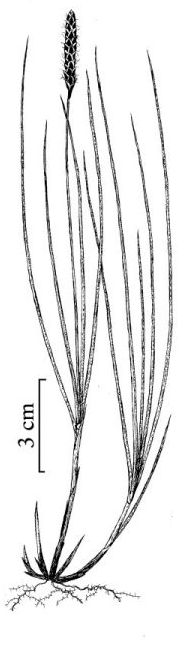
\includegraphics[scale=0.3]{images/carex.png}} \\
    Carex scirpoidea var. convoluta & \\
    Carex scirpoidea subsp. convoluta & \\
    Carex scirpoidea convoluta Kükenth. & \\
    Carex scirpoidea var. convoluta Kuk. & \\
    Carex scirpoidea var. convoluta Kük. & \\
    Carex scirpoidea var. convoluta Kükenth. & \\
    Carex scirpoidea var. convoluta Kükenthal & \\
    Carex scirpoidea Michx. var. convoluta Kük. & \\
    Carex scirpoidea ssp. convoluta (Kük.) Dunlop & \\
    Carex scirpoidea Michx. var. convoluta Kükenth. & \\
    Carex scirpoidea subsp. convoluta (Kük.) Dunlop & \\
    Carex scirpoidea ssp. convoluta (Kukenth.) Dunlop & \\
    Carex scirpoidea Michaux var. convoluta Kükenthal & \\
    Carex scirpoidea subsp. convoluta (Kük.) D.A.Dunlop & \\
    Carex scirpoidea subsp. convoluta (Kük.) D.A. Dunlop & \\
    Carex scirpoidea Michx. ssp. convoluta (Kük.) Dunlop & \\
    Carex scirpoidea subsp. convoluta (Kuk.) D. A. Dunlop & \\
    Carex scirpoidea Michx. subsp. convoluta (Kük.) Dunlop & \\
    Carex scirpoidea Michx. ssp. convoluta (Kükenth.) Dunlop & \\
    Carex scirpoidea subsp. convoluta (Kükenthal) D.A. Dunlop & \\
    Carex scirpoidea Michx. subsp. convoluta (Kük.) D.A.Dunlop & \\
    Carex scirpoidea Michx. subsp. convoluta (Kük.) D.A. Dunlop & \\
    Carex scirpoidea subsp. convoluta (Kükenthal 1909) D.A. Dunlop 1998 & \\
    \hline
    \end{tabular}
  \end{center}
\end{table}

Due to intrinsic diversity of name-strings (Table~\ref{table:carex}) an exact
string matching is not powerful enough to link distributed big data via
scientific names. This problem can be addressed by promoting a rigid standard
restricting each name to a single name-string, or through
\textit{reconciliation}. The former strategy would require a costly
international coordination, would not eliminate future human mistakes, it
cannot be applied to older documents, does not allow for multiple points of
view, nor for changes in taxonomic perspective.

The reconciliation process involves folding of all known name-strings into
lexical groups. This requires that we collate all variant spellings of names.
Parsing is crucial for creating lexical groups of name-strings: it allows to
find the most common denominator of spelling variants -- a canonical form
(\textit{Carex scirpoidea convoluta} in case of Table~\ref{table:carex}) and
extract other important for reconciliation  information (infraspecific ranks,
original and combination authorities etc.). Lexical groups would then require
another level of folding into reconciliation groups where homotypic and
heterotypic synonyms are placed together. This process requires an accurate
database of nomenclatural events (for example Global Names Usage Bank
\cite{Pyle2003}).

Reconciliation uses the most stable component of a name-string -- its canonical
form. Such approach brings us to another problem -- the same canonical form may
be used for more than one taxon or concept in case of homonyms, chresonyms, or
ranks of infraspecies. Analysis of ranks and the authors found by a
parser in name-strings helps to separate homonyms and similar names from each
other.

The next challenge is to replace outdated names with ones that are endorsed by
taxonomic authorities -- this is a process referred to as \textit{resolution}.
Resolution requires an up to date high quality taxonomic and nomenclatural
service (for example catalogue of Life \cite{col}) to map a reconciled
name-string to the currently used name/names. A reconciliation of name-strings
used by a taxonomic authority with name-strings supplied by user makes parsing
a very important step at this stage as well.

A significant number of biodiversity informatics projects (Encyclopedia of Life
\cite{eol}, Global Biodiversity Informatics Facility \cite{gbif}, Catalogue of
Life \cite{col}, World Register of Marine Species \cite{worms}, iDigBio
\cite{idigbio}, VertNet \cite{vertnet} etc.) aggregate information from many
different sources.  Resulting name-strings are inconsistent in their format.
Parsed names can be normalized to the same style. Some name strings are not
properly formed, other contain annotations which are not part of the name.
There are also “surrogate names” -- they depict organisms which were not fully
identified and mapped to a formally described taxon, instead they were
associated with a name string that narrows down identification choices to some
higher clade. Parser helps to recognize such names and mark them as surrogate
name-strings.

After collecting parsed data from a large name-string repository a researcher
can use the data as a basis for statistical analysis, or for practical
purposes. For example parsed data can be used to introduce faceted search by
authors name, year of publication, species epithet etc. If a name-string cannot
be ingested by a high quality parser, the string is almost certainly not a
well-formed scientific name. As a result parser can weed out problematic name
strings from a collection.

\subsection*{Prior Art}

Until recently the problem of scientific name parsing had been addressed by
home-grown scripts running regular expressions or by manual splitting of a name
into its canonical form and the authorship part. Both approaches proved to be
limited. Regular expressions are not designed for recursive patterns (and
complex scientific name strings are recursive by nature, as it is most obvious
with hybrid formulae). Manual approach of splitting names into 2 parts is
expensive, slow, inflexible and cannot elegantly deal with name-strings where
authorship is present in the middle of the name.

Names can be quite complex (for example ``\textit{Brassica oleracea} L.
\textit{subsp.  capitata} (L.) DC. \textit{convar. fruticosa} (Metzg.) Alef.
$\times$ \textit{B. oleracea} L.  \textit{subsp. capitata} (L.) \textit{var.
costata} DC.'')  and include authorship for every mentioned taxon, include or
omit infraspecific ranks, original and combination authors etc. Authorship
itself is quite complex and can include original authors who described a name,
authors of a new combination, or authors who made a name, but did not publish
it. We obviously do not want to exclude names from biodiversity informatics
just because they are not simple enough. We need an approach that is able to
deal with names of any complexity.

In 2008 we decided to create a specialized parsing library
``\textit{biodiversity}'' \cite{biodiversity} written in Ruby and based on
Parsing Expression Grammar (PEG) methodology \cite{Ford2004}. We used an
excellent TreeTop Ruby library \cite{treetop} as an underlying PEG
implementation. PEG is well suited for recursive texts with formally defined
grammars. Scientific names follow rules of nomenclatural codes, and therefore
order and capitalization of elements in scientific names are well structured.

We found that PEG approach allows us to solve all these complexity gracefully.
Also PEG gave us enough flexibility to incorporate edge cases and common
mistakes in formation of names. The library \textit{biodiversity} enjoyed
noticeable popularity. At the time of writing it had been downloaded more than
150,000 times \cite{bdiv_downloads}, it is used by many taxon name resolution
projects (for example by Canadian Register of Marine Species (CARMS)
\cite{carms}, the iPlant TNRS \cite{iplant}, World Registry of Marine Species
(WoRMS) \cite{worms}.  According to BioRuby statistics \textit{biodiversity}
parser is the most popular bio-library in Ruby language \cite{biogems}.

We consider \textit{biodiversity} parser library to be a working prototype -- a
playground which allowed us to identify parsing problems and implement
solutions for them. In the process we found that Parsing Expression Grammar is
very well suited for breaking scientific names into semantic elements. In 2015
we decided to use everything we learned and write ``\textit{gnparser}'' a
completely new parser in Scala to achieve significant boost in speed,
scalability and portability of the library. In this manuscript we describe
features, performance and discuss future enhancements of this new parser.

\section*{Implementation}

- existing language classes: regular languages, Deterministic context-free languages, Parsing expression grammars, General context-free. Why PEGs?

- existing implementations of PEG parser generator % https://en.wikipedia.org/wiki/Comparison_of_parser_generators}

- existing combinator parsers. written in parboiled2/Scala. What was the reason for the choice?

- gnparser consists of three parts. Short description of parts

\subsection*{Parser}

- explanation of functionality: parser engine

- dependency of the rest 2 components on this one

- versions of scala supported

- relation to biodiversity parserj

- relationship to parboiled2, mention Alex' role in paraboiled2

- patches to parboiled2 (+ links to human-readable explanation: blog or published paper)

- bottlenecks optimizations in parser

- input: name string(s), output: JSON object.

- Figure with output example and short explanation

- Quality output -- short explanation.

- reference to JSON schema (attachment), simple explanation of fields
(attachment)

- short explanations of tests. Connection between tests and schema

- usage with other languages as a library

\subsection*{Runner}

- explanation of functionalilty: command line tool, socket server

- command line tool -- input for one name, output, intput for file, output

- socket server -- very short explanation how it runs. Input, Output

- mention parallelization in parsing

- TODO: should we change input output to be more similar to REST API?
  Make it JSON array of names as input, array of gnparser objects as output

\subsection*{Web}

- explanation of functionality: Web GUI, REST API

- input and output for API use via GET and POST

\subsection*{Installation}

- reference to README. Reference and short explanation of the Docker project
(in attachments)

- MIT license

\subsection*{Testing Methods}

Data for our tests were randomly chosen from 24 million name-strings of the
Global Names Index. These resulting datasets consisted of strings acquired
from a variety of data sources and were a mixture of well-formed names, names
with formatting and spelling mistakes, and non-name strings misrepresented as
names.

We compared performance of gnparser with 2 other projects -- Biodiversity
parser\cite{biodiversity} (also developed by Global Names), and GBIF
name-parser\cite{gbifNameParser}. Another project we considered was YASMEEN
parser from iMarine\cite{VandenBerghe2015}, however we found that with our
dataset it generated dramatically more mistakes than other parsers
($Precision$ 0.534, $Recall$ 1.0, $F1$ 0.6962), and we decided to exclude it
from the tests.

To find out the throughput of parsing we used a computer with Intel i7-4930K
CPU (6 cores, 12 threads, at 3.4 GHz), 64GB of memory, and 250GB Samsung 840
EVO SSD, running Ubuntu version 14.04. Throughput was determined by processing
of 1,000,000 random name-strings from GNI.

To study effects of parallel execution on throughput we used
\textit{ParallelParser} class from Biodiversity parser and \textit{gnparse}
command line interface for gnparser. For GBIF name-parser we created a thin
wrapper with multi-threaded capabilities\cite{gbifparser}.

For determining $Precision$, $Recall$ and $Accuracy$ of parsed names the
dataset size was 1000 name-strings. To estimate quality for all parsers we
needed to pick a feature which is common for all three of them and is a good
indicator of performance.  We decided to use a combination of canonical form
and terminal authorship.  Canonical form represents the most stable elements
of a name, while terminal authorship corresponds to the authority of the most
detailed element of the name. For example in "\textit{Oriastrum lycopodioides}
Wedd.  var.  \textit{glabriusculum} Reiche" canonical form is
"\textit{Oriastrum lycopodioides glabriusculum}" and terminal authorship is
"Reiche", not "Wedd.".  Algorithms necessary to select components of a
canonical form of a name and to find the terminal authorship are good
indicators of a parser quality.

When both the canonical form and the terminal authorship were determined
correctly we marked the result as true positive ($\text{tp}$).  If one or both
of them were determined incorrectly -- the result was marked a false positive
($\text{fp}$). Correctly discarded from parsing name-strings were marked as
true negatives ($\text{tn}$). False negatives ($\text{fn}$) were "suitable"
name-strings which should be parsed, but were nevertheless discarded.

Some names in the dataset were not well-formed. If a human could extract the
canonical form and the terminal authorship from them we did count them.
Examples of such name-strings are \textbf{"Bumetopia (bumetopia)
quadripunctata Breuning"} (low case subgenus), \textbf{"Campylium gollanii C.
M?ller ex Vohra 1970 [1972]"} (miscoded UTF-8 symbol and additional year in
square brackets), \textbf{"Myosorex muricauda (Miller, 1900)."} (period after
authorship).

$Precision$ is a percentage of names parsed correctly and is calculated as

\[Precision = \dfrac{\text{tp}}{(\text{tp} + \text{fp})}\]

$Recall$ is a percentage of names detected and is calculated as

\[Recall = \dfrac{\text{tp}}{(\text{tp} + \text{fn})}\]

$F1-measure$ is a balanced harmonic mean (where $Precision$ and $Recall$ have
the same weight). When both $Precision$ and $Recall$ vary, $F1-measure$ allows
to compare results nevertheless. It is calculated as

\[F1 = \dfrac{2 \times Precision \times Recall}{(Precision + Recall)}\]

$Accuracy$ is a percentage of correct results. It is calculated as

\[Accuracy = \dfrac{\text{tp} + \text{tn}}
  {\text{tp} + \text{tn} + \text{fp} + \text{fn}}\]

Validity of names was not taken into account, as it is out of scope of
parsers' functionality. For example in case of a name-string \textbf{"Example
name Word var.  something Capitalized Words, 1900"}, canonical form
\textbf{"Example name something"} and terminal authorship \textbf{"Capitalized
Words, 1900"} would be considered a true positive.

It is important for parser to accurately distinguish between strings of
scientific names, names of viruses, surrogate names, and non-names. To find
out how well parsers distinguished strings which are not scientific names, we
calculated $Precision$ for discarded/non-parsed strings. If done correctly
not-parsed strings would include only names of viruses and non-scientific
names.

We processed 100,000 name-strings by each parser, and found that about 1000 of
them had been discarded as not-parseable. $Precision$ in this case showed
percentage of correctly discarded names.  We do not know $Recall$, as it was
not feasible to manualy find it for 100,000 names. To get a glimpse on names
which had to be discarded, but were parsed instead we analysed intersections
and differences of the results between the three parsers.

\section*{Results and Discussion}

The goal of Global Names Architecture is creation of an infrastructure for
biology which uses scientific names to connect and inter-exchange biological
data in the most complete, accurate and painless way. Parsing is the first
step to this goal. We believe a scienific name parser needs to correspond to
the following requirements to be up to the task:

1. \textbf{High Quality}. A parser should be able to break names into their
semantic elements on a level of a trained nomenclator or better. When we are
able to reach this goal we become independent on how names are stored in
various databases and be limited to databases where names are parsed by humans
or to exact string matching. Moreover, the advent of high quality parsers
eliminates the need for humans to perform this very expensive, tedious and
error-prone task.

2. \textbf{Global Scope}. Parser should be able to support all types of
scientific names, including the most complex ones -- hybrid formulae,
multi-infraspecific names, names with multilevel authorships etc. Without
parsing, the ability to find the same name in different sources is severely
diminished and valuable information attached to scientific names is hidden
from researchers.

3. \textbf{Parsing Completeness}. All information included into a name is
important, not only canonical form. Authorship, year, rank information allows
to distinguish homonyms, similar names, synonyms, spelling mistakes,
chresonyms from each other, narrowing the search down to relevant information.
From other side it allows people who manage large collections of names to weed
out mistakes and increase quality of their databases.

4. \textbf{Speed}. For Global Names Architecture purposes a parser needs to be
fast and effective to satisfy needs of users everywhere on the globe.  High
throughput of parsing becomes very important: on one side it increases speed
with which people will receive requested information, on another side it
directly influences the cost of required hardware, as well as the cost of
hardware upgrades.

5. \textbf{Accessibility}. Open source approach shines the most when it covers
the widest possible audience. A parser needs good documentation, ability to
work as a library, command line tool, tool with graphical interface, run as
socket and RESTful service.

Further we are going to talk about gnparser from the point of these 5
requirements

\subsection*{High quality parsing}

High quality parsing is probaby the most important out of the 5 requirements.
We tested gnparser together with 2 other parsing projects. To our knowledge
these three represent state of the art for parsing biological scientific
names. GBIF name-parser uses regular expressions approach, while gnparser and
biodiversity parser use PEG approach. Results for our quality measurements are
shown in Table~\ref{table:precision}.

When data contain large proportion of true negatives ($\text{tn}$) $Accuracy$
is not a good measure, as it would favor algorithms which distinquish negative
results, rather than finding positive ones. However in our case datasets had
only $\approx1\%$ of non-scientific names, true negatives were rare and had
very little influence on results. $Recal$ for all parsers was very high, which
means false negatives had insignificant influence on results as well. Taking
this in account we think $Accuracy$ is the best measure for our tests and
is sufficient to compare quality for all cases.

Altogether we find that all 3 parsers performed very well with $Accuracy$
higher than $95\%$. Both gnparser and biodiversity parser were approaching
99\% mark. Moreover, most of the false positives came from names with
mistakes. For example, out of 11 false positives for gnparser only 2 were
well-formed names:

\begin{verbatim}
    Eucalyptus subser. Regulares Brooker
    Jacquemontia spiciflora (Choisy) Hall. fil.

    Acanthocephala declivis variety guianensis Osborn, 1904
    Atysa (?) frontalis
    Bumetopia (bumetopia) quadripunctata Breuning, 1950
    Cyclotella kã¼tzingiana Thwaites
    Elaphidion (romaleum) tæniatum Leconte, 1873
    Hieracium nobile subsp. perclusum (Arv. -Touv. ) O. Bolòs & Vigo
    Leptomitus vitreus (Roth) Agardh{?}
    Myosorex muricauda (Miller, 1900).
    Papillaria amblyacis (M<81>ll.Hal.) A.Jaeger
\end{verbatim}

As it is seen from the name-strings above we do expect parsers to deal with
mistakes, annotations, and unicode characters miscodings. To alert users
about them gnparser has a unique feature of generating warnings for each found
problem in a name-string.

When parsers reach $\approx80\%$ $Accuracy$ they hit a "long tail" of problems
where each particular case of wrong parsing is rare, and every new manual test
against 1,000-10,000 name-strings reveals new issues. For all three parsers
developer teams performed a meticulous task of adding one rare case after
another to the list of problems and finding ways to incoporate solutions.
Parsing problems found during preparation of this paper will be solved in the
next version of gnparser as well. Quality of parsing rules is constantly
improving, in our estimation gnparser can reach $\textgreater 99.5\% Accuracy$
without diminishing $Recall$.

During incorporation of new rules to increase $Recall$ it is important to
judge if there is a risk of bringing down $Precision$ by introducing new false
positives.  For example GBIF name-parser allows genus of a name-string to
start with a lowercase character. As a result the strings below were parsed as
scientific names, while other parsers ignored them:


\begin{verbatim}
    acid mine drainage metagenome
    agricultural soil bacterium CRS5639T18-1
    agricultural soil bacterium SC-I-8
    algal symbiont of Cladonia variegata MN075
    alpha proteobacterium AP-24
    anaerobic bacterium ANA No.5
    anoxygenic photosynthetic bacterium G16
    archaeon enrichment culture clone AOM-SR-A23
    bacterium endosymbiont of Plateumaris fulvipes
    bacterium enrichment culture DGGE band 61_3_FG_L
    barley rhizosphere bacterium JJ-220
    bovine rumen bacterium niuO17
\end{verbatim}

Solutions like these might increase $Recall$ for certain low-quality datasets,
but as we see in this example they also decrease $Precision$ for other, better
quality datasets. When dealing with "dirty" datasets with very predictable
problems (like lowercase genus) we recommend to write a preparser script which
"normalizes" known problems and then use a high quality parser.

Our testing also revealed differences between regular expressions and PEG
approaches. Our results show that both can achieve high quality results for
finding canonical forms, but regular expressions approach is less suitable for
more complex name-strings. The reason for this is recursive nature of
scientific names.  It is relatively easy to parse simpler structured
name-strings with regular expressions, but for more involved name-strings
complications arise from the recursive nature of names. At some point these
complications become unsurmantable.

\subsection*{Global Scope}

If we want to trully connect biological data using scientific names, no names
should be left behind, no matter how complex they are. During out testing we
found that $Accuracy$ of GBIF name-parser was negatively affected by not
dealing with hybrid formulae and infrasubspecific names (names with more then
one infraspecific epithet). Regular expressions do not support recursion --
the more complex names are, the harder it becomes to parse them. For example
the following names were not supported by GBIF name-parser:

\begin{verbatim}
    Crataegus chlorosarca subtaxon pubescens E.L.Wolf
    Erigeron peregrinus ssp.callianthemus var. eucallianthemus
    Salvelinus fontinalis x Salmo gairdneri
    Echinocereus fasciculatus var. bonkerae × E. fasciculatus
      var. fasciculatus
\end{verbatim}

We use PEG approach because it allows to nest parsing rules within each other,
making it possible to create progressively more and more complex rules -- the
first rule just defines what space is, the last rule defines hybrid formulas.
Such support for recursion allows gnparser to handle full spectrum of
scientific names.

\begin{table}[htb]
  \begin{center}
    \caption{Precision/Recall for processed by parsers 1000
    name-strings}\label{table:precision}
    \begin{tabular}{|l|*{3}{l}|}
      \hline
                             & gnparser & gbif-parser & biodiversity \\
      \hline
      \textit{True Positive} & 976      & 955         & 971          \\
      \textit{True Negative} & 13       & 12          & 13           \\
      \textit{False Positive}& 11       & 32          & 16           \\
      \textit{False Negative}& 0        & 1           & 0            \\
      \textit{Precision}     & 0.9888551& 0.967578    & 0.9837893    \\
      \textit{Recall}        & 1.0      & 0.998954    & 1.0          \\
      \textit{F1}            & 0.9943963& 0.983016    & 0.9918284    \\
      \textit{Accuracy}      & 0.989    & 0.967       & 0.984        \\
      \hline
    \end{tabular}
  \end{center}
\end{table}

\begin{table}[htb]
  \begin{center}
    \caption{Precision for discarded by parsers names, out of 100 000
    name-strings}\label{table:unparsed}
    \begin{tabular}{|l|*{3}{l}|}
      \hline
                              & gnparser & gbif-parser & biodiversity \\
      \hline
      \textit{Total discarded}& 1131     & 1082        & 1161         \\
      \textit{True Positive}  & 1129     & 940         & 1152         \\
      \textit{False Positive} & 2        & 142         & 9            \\
      \textit{Precision}      & 0.998231 & 0.868761    & 0.9922481    \\
      \hline
    \end{tabular}
  \end{center}
\end{table}

\begin{figure}[htbp]
  \begin{center}
    \caption{
      Names parsed per second by GN, GBIF and Biodiversity parsers
      (runing on 1-12 parallel threads).
    }\label{figure:throughput}
    \vspace{0.5cm}
    \begin{tabular}{| l | *{3}{r} | c c c |}
      \hline
      \multirow{1}{*}Threads & gnparser & gbif-paser & biodiversity
      & \multicolumn{3}{c |}{Ratio} \\
      \cline{5-7}
      & & & & gn & gbif & bio \\
      \hline
      1  & 5944  & 6389  & 1111 & 1 & 1.07 & 0.19 \\
      2  & 11416 & 12638 & 1722 & 1 & 1.11 & 0.14 \\
      4  & 20500 & 21994 & 2556 & 1 & 1.07 & 0.12 \\
      8  & 24805 & 30972 & 2777 & 1 & 1.25 & 0.11 \\
      12 & 26055 & 31833 & 2527 & 1 & 1.22 & 0.10 \\
      \hline
    \end{tabular}
    % Created by tikzDevice version 0.9 on 2015-12-21 16:35:00
% !TEX encoding = UTF-8 Unicode
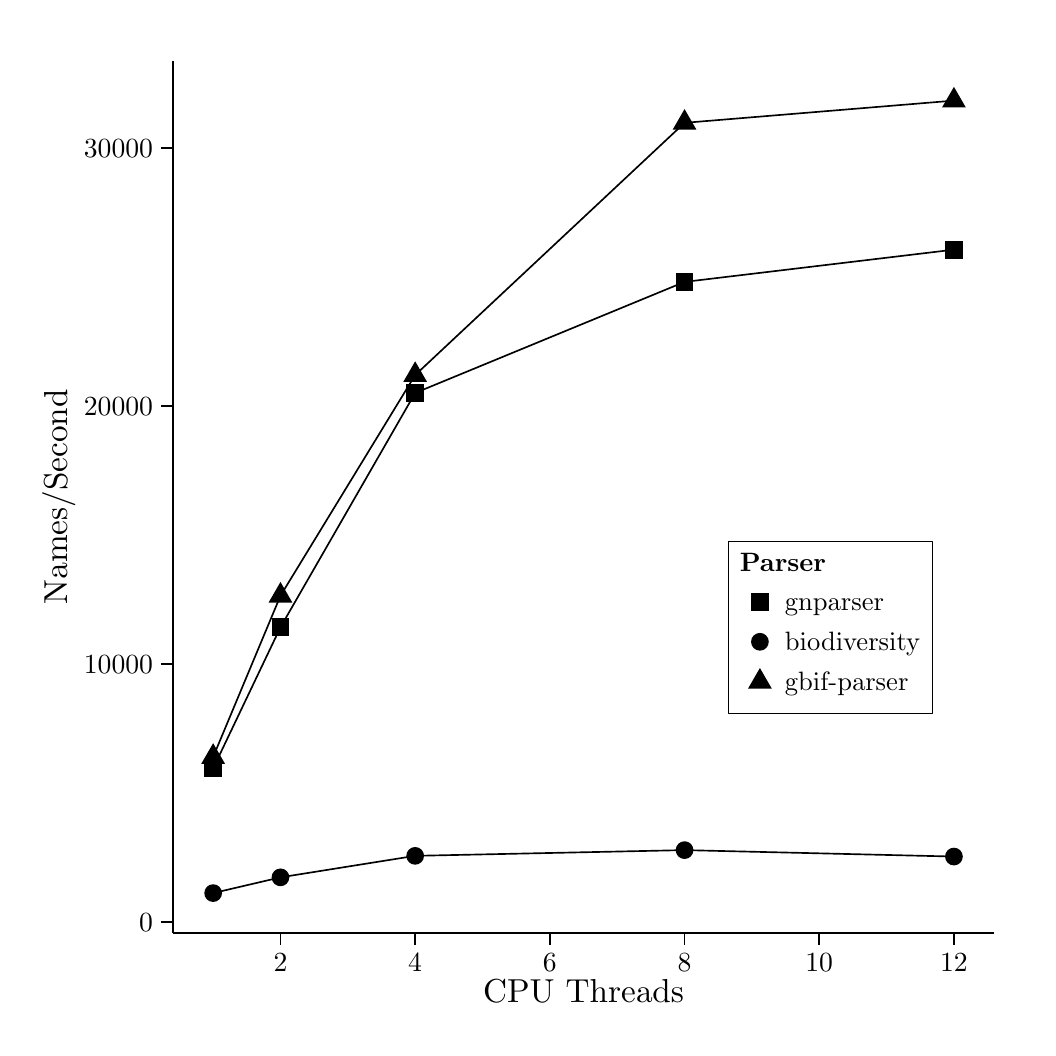
\begin{tikzpicture}[x=1pt,y=1pt]
\definecolor{fillColor}{RGB}{255,255,255}
\path[use as bounding box,fill=fillColor,fill opacity=0.00] (0,0) rectangle (361.35,361.35);
\begin{scope}
\path[clip] (  0.00,  0.00) rectangle (361.35,361.35);
\definecolor{drawColor}{RGB}{255,255,255}
\definecolor{fillColor}{RGB}{255,255,255}

\path[draw=drawColor,line width= 0.6pt,line join=round,line cap=round,fill=fillColor] (  0.00,  0.00) rectangle (361.35,361.35);
\end{scope}
\begin{scope}
\path[clip] ( 52.42, 34.31) rectangle (349.30,349.30);
\definecolor{fillColor}{RGB}{255,255,255}

\path[fill=fillColor] ( 52.42, 34.31) rectangle (349.30,349.30);
\definecolor{drawColor}{RGB}{255,255,255}

\path[draw=drawColor,line width= 0.6pt,line join=round] ( 52.42, 38.27) --
	(349.30, 38.27);

\path[draw=drawColor,line width= 0.6pt,line join=round] ( 52.42,131.48) --
	(349.30,131.48);

\path[draw=drawColor,line width= 0.6pt,line join=round] ( 52.42,224.69) --
	(349.30,224.69);

\path[draw=drawColor,line width= 0.6pt,line join=round] ( 52.42,317.90) --
	(349.30,317.90);

\path[draw=drawColor,line width= 0.6pt,line join=round] ( 91.35, 34.31) --
	( 91.35,349.30);

\path[draw=drawColor,line width= 0.6pt,line join=round] (140.02, 34.31) --
	(140.02,349.30);

\path[draw=drawColor,line width= 0.6pt,line join=round] (188.69, 34.31) --
	(188.69,349.30);

\path[draw=drawColor,line width= 0.6pt,line join=round] (237.36, 34.31) --
	(237.36,349.30);

\path[draw=drawColor,line width= 0.6pt,line join=round] (286.03, 34.31) --
	(286.03,349.30);

\path[draw=drawColor,line width= 0.6pt,line join=round] (334.70, 34.31) --
	(334.70,349.30);
\definecolor{drawColor}{RGB}{0,0,0}

\path[draw=drawColor,line width= 0.6pt,line join=round] ( 67.02, 48.63) --
	( 91.35, 54.32) --
	(140.02, 62.09) --
	(237.36, 64.16) --
	(334.70, 61.83);

\path[draw=drawColor,line width= 0.6pt,line join=round] ( 67.02, 97.82) --
	( 91.35,156.08) --
	(140.02,235.82) --
	(237.36,326.96) --
	(334.70,334.99);

\path[draw=drawColor,line width= 0.6pt,line join=round] ( 67.02, 93.68) --
	( 91.35,144.69) --
	(140.02,229.35) --
	(237.36,269.48) --
	(334.70,281.13);
\definecolor{fillColor}{RGB}{0,0,0}

\path[fill=fillColor] ( 63.82, 90.48) --
	( 70.22, 90.48) --
	( 70.22, 96.88) --
	( 63.82, 96.88) --
	cycle;

\path[fill=fillColor] ( 88.15,141.48) --
	( 94.55,141.48) --
	( 94.55,147.89) --
	( 88.15,147.89) --
	cycle;

\path[fill=fillColor] (136.82,226.15) --
	(143.22,226.15) --
	(143.22,232.55) --
	(136.82,232.55) --
	cycle;

\path[fill=fillColor] (234.16,266.28) --
	(240.56,266.28) --
	(240.56,272.68) --
	(234.16,272.68) --
	cycle;

\path[fill=fillColor] (331.50,277.93) --
	(337.90,277.93) --
	(337.90,284.33) --
	(331.50,284.33) --
	cycle;

\path[fill=fillColor] ( 67.02,102.80) --
	( 71.33, 95.33) --
	( 62.71, 95.33) --
	cycle;

\path[fill=fillColor] ( 91.35,161.06) --
	( 95.66,153.59) --
	( 87.04,153.59) --
	cycle;

\path[fill=fillColor] (140.02,240.80) --
	(144.33,233.33) --
	(135.71,233.33) --
	cycle;

\path[fill=fillColor] (237.36,331.94) --
	(241.67,324.47) --
	(233.05,324.47) --
	cycle;

\path[fill=fillColor] (334.70,339.96) --
	(339.01,332.50) --
	(330.39,332.50) --
	cycle;

\path[fill=fillColor] ( 67.02, 48.63) circle (  3.20);

\path[fill=fillColor] ( 91.35, 54.32) circle (  3.20);

\path[fill=fillColor] (140.02, 62.09) circle (  3.20);

\path[fill=fillColor] (237.36, 64.16) circle (  3.20);

\path[fill=fillColor] (334.70, 61.83) circle (  3.20);
\end{scope}
\begin{scope}
\path[clip] (  0.00,  0.00) rectangle (361.35,361.35);
\definecolor{drawColor}{RGB}{0,0,0}

\path[draw=drawColor,line width= 0.6pt,line join=round] ( 52.42, 34.31) --
	( 52.42,349.30);
\end{scope}
\begin{scope}
\path[clip] (  0.00,  0.00) rectangle (361.35,361.35);
\definecolor{drawColor}{RGB}{0,0,0}

\node[text=drawColor,anchor=base east,inner sep=0pt, outer sep=0pt, scale=  1.00] at ( 45.30, 34.83) {0};

\node[text=drawColor,anchor=base east,inner sep=0pt, outer sep=0pt, scale=  1.00] at ( 45.30,128.04) {10000};

\node[text=drawColor,anchor=base east,inner sep=0pt, outer sep=0pt, scale=  1.00] at ( 45.30,221.25) {20000};

\node[text=drawColor,anchor=base east,inner sep=0pt, outer sep=0pt, scale=  1.00] at ( 45.30,314.46) {30000};
\end{scope}
\begin{scope}
\path[clip] (  0.00,  0.00) rectangle (361.35,361.35);
\definecolor{drawColor}{RGB}{0,0,0}

\path[draw=drawColor,line width= 0.6pt,line join=round] ( 48.15, 38.27) --
	( 52.42, 38.27);

\path[draw=drawColor,line width= 0.6pt,line join=round] ( 48.15,131.48) --
	( 52.42,131.48);

\path[draw=drawColor,line width= 0.6pt,line join=round] ( 48.15,224.69) --
	( 52.42,224.69);

\path[draw=drawColor,line width= 0.6pt,line join=round] ( 48.15,317.90) --
	( 52.42,317.90);
\end{scope}
\begin{scope}
\path[clip] (  0.00,  0.00) rectangle (361.35,361.35);
\definecolor{drawColor}{RGB}{0,0,0}

\path[draw=drawColor,line width= 0.6pt,line join=round] ( 52.42, 34.31) --
	(349.30, 34.31);
\end{scope}
\begin{scope}
\path[clip] (  0.00,  0.00) rectangle (361.35,361.35);
\definecolor{drawColor}{RGB}{0,0,0}

\path[draw=drawColor,line width= 0.6pt,line join=round] ( 91.35, 30.04) --
	( 91.35, 34.31);

\path[draw=drawColor,line width= 0.6pt,line join=round] (140.02, 30.04) --
	(140.02, 34.31);

\path[draw=drawColor,line width= 0.6pt,line join=round] (188.69, 30.04) --
	(188.69, 34.31);

\path[draw=drawColor,line width= 0.6pt,line join=round] (237.36, 30.04) --
	(237.36, 34.31);

\path[draw=drawColor,line width= 0.6pt,line join=round] (286.03, 30.04) --
	(286.03, 34.31);

\path[draw=drawColor,line width= 0.6pt,line join=round] (334.70, 30.04) --
	(334.70, 34.31);
\end{scope}
\begin{scope}
\path[clip] (  0.00,  0.00) rectangle (361.35,361.35);
\definecolor{drawColor}{RGB}{0,0,0}

\node[text=drawColor,anchor=base,inner sep=0pt, outer sep=0pt, scale=  1.00] at ( 91.35, 20.31) {2};

\node[text=drawColor,anchor=base,inner sep=0pt, outer sep=0pt, scale=  1.00] at (140.02, 20.31) {4};

\node[text=drawColor,anchor=base,inner sep=0pt, outer sep=0pt, scale=  1.00] at (188.69, 20.31) {6};

\node[text=drawColor,anchor=base,inner sep=0pt, outer sep=0pt, scale=  1.00] at (237.36, 20.31) {8};

\node[text=drawColor,anchor=base,inner sep=0pt, outer sep=0pt, scale=  1.00] at (286.03, 20.31) {10};

\node[text=drawColor,anchor=base,inner sep=0pt, outer sep=0pt, scale=  1.00] at (334.70, 20.31) {12};
\end{scope}
\begin{scope}
\path[clip] (  0.00,  0.00) rectangle (361.35,361.35);
\definecolor{drawColor}{RGB}{0,0,0}

\node[text=drawColor,anchor=base,inner sep=0pt, outer sep=0pt, scale=  1.20] at (200.86,  9.03) {CPU Threads};
\end{scope}
\begin{scope}
\path[clip] (  0.00,  0.00) rectangle (361.35,361.35);
\definecolor{drawColor}{RGB}{0,0,0}

\node[text=drawColor,rotate= 90.00,anchor=base,inner sep=0pt, outer sep=0pt, scale=  1.20] at ( 14.29,191.81) {Names/Second};
\end{scope}
\begin{scope}
\path[clip] (  0.00,  0.00) rectangle (361.35,361.35);
\definecolor{drawColor}{RGB}{0,0,0}
\definecolor{fillColor}{RGB}{255,255,255}

\path[draw=drawColor,line width= 0.3pt,line join=round,line cap=round,fill=fillColor] (253.09,113.49) rectangle (326.76,175.63);
\end{scope}
\begin{scope}
\path[clip] (  0.00,  0.00) rectangle (361.35,361.35);
\definecolor{drawColor}{RGB}{0,0,0}

\node[text=drawColor,anchor=base west,inner sep=0pt, outer sep=0pt, scale=  0.96] at (257.36,164.73) {\bfseries Parser};
\end{scope}
\begin{scope}
\path[clip] (  0.00,  0.00) rectangle (361.35,361.35);
\definecolor{drawColor}{RGB}{255,255,255}
\definecolor{fillColor}{RGB}{255,255,255}

\path[draw=drawColor,line width= 0.6pt,line join=round,line cap=round,fill=fillColor] (257.36,146.67) rectangle (271.82,161.12);
\end{scope}
\begin{scope}
\path[clip] (  0.00,  0.00) rectangle (361.35,361.35);
\definecolor{fillColor}{RGB}{0,0,0}

\path[fill=fillColor] (261.39,150.69) --
	(267.79,150.69) --
	(267.79,157.09) --
	(261.39,157.09) --
	cycle;
\end{scope}
\begin{scope}
\path[clip] (  0.00,  0.00) rectangle (361.35,361.35);
\definecolor{drawColor}{RGB}{255,255,255}
\definecolor{fillColor}{RGB}{255,255,255}

\path[draw=drawColor,line width= 0.6pt,line join=round,line cap=round,fill=fillColor] (257.36,132.21) rectangle (271.82,146.67);
\end{scope}
\begin{scope}
\path[clip] (  0.00,  0.00) rectangle (361.35,361.35);
\definecolor{fillColor}{RGB}{0,0,0}

\path[fill=fillColor] (264.59,139.44) circle (  3.20);
\end{scope}
\begin{scope}
\path[clip] (  0.00,  0.00) rectangle (361.35,361.35);
\definecolor{drawColor}{RGB}{255,255,255}
\definecolor{fillColor}{RGB}{255,255,255}

\path[draw=drawColor,line width= 0.6pt,line join=round,line cap=round,fill=fillColor] (257.36,117.76) rectangle (271.82,132.21);
\end{scope}
\begin{scope}
\path[clip] (  0.00,  0.00) rectangle (361.35,361.35);
\definecolor{fillColor}{RGB}{0,0,0}

\path[fill=fillColor] (264.59,129.96) --
	(268.90,122.50) --
	(260.28,122.50) --
	cycle;
\end{scope}
\begin{scope}
\path[clip] (  0.00,  0.00) rectangle (361.35,361.35);
\definecolor{drawColor}{RGB}{0,0,0}

\node[text=drawColor,anchor=base west,inner sep=0pt, outer sep=0pt, scale=  0.96] at (273.62,150.59) {gnparser};
\end{scope}
\begin{scope}
\path[clip] (  0.00,  0.00) rectangle (361.35,361.35);
\definecolor{drawColor}{RGB}{0,0,0}

\node[text=drawColor,anchor=base west,inner sep=0pt, outer sep=0pt, scale=  0.96] at (273.62,136.13) {biodiversity};
\end{scope}
\begin{scope}
\path[clip] (  0.00,  0.00) rectangle (361.35,361.35);
\definecolor{drawColor}{RGB}{0,0,0}

\node[text=drawColor,anchor=base west,inner sep=0pt, outer sep=0pt, scale=  0.96] at (273.62,121.68) {gbif-parser};
\end{scope}
\end{tikzpicture}

  \end{center}
\end{figure}

\subsection*{Parsing Completness}

By far extraction of canonical form is the most useful and the most practiced
parsing technique. However it is not enough, because canonical form does not
determine a name completely. In the example from Table~\ref{table:carex}
\textbf{Carex scirpoidea convoluta} is a canonical form for \textbf{Carex
scirpoidea var. convoluta Kükenthal} and \textbf{Carex scirpoidea ssp.
convoluta (Kük.) Dunlop}. In the first case name string describes a variety
\textbf{convoluta} of \textbf{Carex scirpoidea} species described by
\textbf{Kükenthal}. In the second case \textbf{Dunlop} recategorized \textbf
{convoluta} as subspecies of \textbf{Carex scirpoidea}. We would not be able
to distinguish between these two different names without seing a rank of a
name and the corresponding authorship. Furthermore it was important to see in
the second example that \textbf{(Kük.)} was original author and
\textbf{Dunlop} was the author of the new combination.

After the match by canonical form is done, ranks, authors, and "types" of
authorship allow to distinguish similar names from each other.
Name-string \textbf{Carex scirpoidea Michx. var. convoluta Kükenth.} gives
additional clue that we talk about \textbf{Carex scirpoidea} species described
by \textbf{Michx}

All components of a name are important, and need to be parsed and categorized.
With gnparser we describe meaning of every word in the parsed name-string
and present it in JSON format:

\begin{verbatim}
  {"name_string_id":"203213f3-99d1-5f5e-810a-4453c4d220cb", "parsed":true,
  "quality":1, "parser_version":"0.2.0", "verbatim":"Carex scirpoidea Michx.
  subsp. convoluta (Kük.) D.A. Dunlop", "normalized":"Carex scirpoidea Michx.
  ssp. convoluta (Kük.) D. A. Dunlop", "canonical_name":{"value":"Carex
  scirpoidea convoluta", "extended":"Carex scirpoidea ssp. convoluta"},
  "hybrid":false, "surrogate":false, "virus":false,
  "details":[{"genus":{"value":"Carex"},
  "specific_epithet":{"value":"scirpoidea", "authorship":{"value":"Michx.",
  "basionym_authorship":{"authors":["Michx."]}}},
  "infraspecific_epithets":[{"value":"convoluta", "rank":"ssp.",
  "authorship":{"value":"(Kük.) D. A. Dunlop",
  "basionym_authorship":{"authors":["Kük."]},
  "combination_authorship":{"authors":["D. A. Dunlop"]}}}]}],
  "positions":[["genus",0,5], ["specific_epithet",6,16],
  ["author_word",17,23], ["rank",24,30], ["infraspecific_epithet",31,40],
  ["author_word",42,46], ["author_word",48,50], ["author_word",50,52],
  ["author_word",53,59]]}
\end{verbatim}

The output includes detailed meaning of every word in a name, indications if
the name-string was parsed correctly, if it is a virus name, hybrid, or
surrogate. Surrogates are names pointing to a higher clade and ending with
some accession string like \textbf{Coleoptera sp. BOLD:AAV0432}. The output
also includes position of each word in the name-string with attached meaning
of the word.

Last but not least JSON output contains UUID version 5 calculated from the
verbatim name-string. This UUID is guaranteed to be the same for the same
name-string, allowing to globally connect information and annotations to such
UUID.

\subsection*{Parsing Speed}

In our discussion so far there was little difference between biodiversity
parser and gnparser. A dramatic difference appears in their parsing speed and
ability to scale. Parsing speed is important for two reasons. Firstly a user
gets results faster with a faster parser. Secondly if parser is 10 times
faster it means the cost of hardware to run it can be 10 times cheaper for the
same amount of work to be done.

For example, it took us 40 days to find and index names in Biodiversity
Heritage Library. Just parsing step alone took more than a day. When somene
finds a problem with name resolution in BHL, is not feasible to fix it at the
moment, as it would take 40 days of reindexing whole BHL corpus of data. Our
goal is to do this job in 1 day, so when our algorithms improve we can
regularly completely rebuild the BHL scientific name index.

One of the main reasons of rewriting parser from scratch was a necessity to
increase throughput of parsing. Resolution of names is a very common problem
and to solve it well we need to work on removing existing bottlenecks -- one
of the obvious ones is parsing.

Results on the speed performance are given in Figure~\ref{figure:throughput}.
From 1 to 4 CPU threads gnparser and gbif parser showed similar throughput,
while biodiversity parser was ~5 times slower on one thread and ~8 times
slower on 4 threads. GBIF parser scaled better beyond 4 processors and for 12
parallel threads it was 1.22 times faster than gnparser. Both gnparser and
GBIF parser had been significantly faster than biodiversity, and scaled better
as well.

When gnparser runs on 4 CPU threads it performs 8 times faster than
biodiversity parser. It means we need to spend 8 times less on the hardware
using gnparser, and performance-wise we are eliminating a bottleneck of the
parsing step.

\subsection*{Accessibility}

Under accessibility we mean ability of a code to be used by the widest
audience possible. For Open Source projects accessibility is very important,
as the more people use a software the lower is the cost of its creation.

We designed gnparser with accessibility in mind from the start.  Scala
language allows to use gnparser as a library in Scala, Java, Python, JRuby, R,
JavaScript and a great variety of languages based on Java Virtual Machine. If
a user wants to use it in some other language they can connect to the parser
via socket server interface. There is also a command line tool, web interface,
and RESTful API available.

We pay close attention to documentation, trying to keep it detailed, clear and
up to date. We have an extensive test suite which describes parser's behavior
and also is a great source of examples of parser's functionality and output
format.

All this creates larger potential audience for the parser, and will help many
researches and programmers to deal with the complex problem in biodiversity
informatics.

The summary of results and discussion is depicted in
Table~\ref{table:summary}

\begin{table}[htb]
  \begin{center}
    \caption{Summary comparison of Scientific Name Parsers}
    \label{table:summary}
    \begin{tabular}{|l|*{3}{l}|}
      \hline
                             & gnparser & gbif-parser & biodiversity \\
      \hline
      \textit{Accuracy}      & $98.9\%$ & $96.7\%$    & $98.4\%$     \\
      \textit{Hybrid formulas support}      & Yes     & No     & Yes \\
      \textit{Infrasubspecies support}& Yes       & No         & Yes \\
      \textit{Throughput (names/s)}& 5944  & 6389       & 1111         \\
      \textit{Parsing details}     & Complete & Partial    & Complete    \\
      \textit{Library for the same language}    & Yes      & Yes    & Yes \\
      \textit{Library for other languages}            & Yes & Yes    & No    \\
      \textit{Command line tool}      & Yes    & No       & Yes        \\
      \textit{Socket server}      & Yes    & No       & Yes        \\
      \textit{Web Interface}      & Yes    & Yes       & Yes        \\
      \textit{RESTful service}      & Yes    & Yes       & Yes        \\
      \hline
    \end{tabular}
  \end{center}
\end{table}

\subsection*{Future plans}

In the following years we will continue to work on parser and improve its
accuracy and speed. We are planning to build high quality/throughput name
resolution and name finding services, where gnparser will play a key role.
It might be interesting to explore using parsers as a programmatic version
of existing nomenclatural codes and make an automatic quality check for newly
introduced names.

\section*{Conclusions}

We introduced \textit{gnparser}, a tool for dissecting scientific name strings
into meaningful parts. Parsing of name strings is necessary component for their
matching, finding them in texts, sharing them in standardised forms,
extracting, comparing and analysing metadata ``hidden'' in the name strings.
The gnparser tool is released under MIT Open Source license, contains command
line executable, socket, web, and REST services, and is optimized for use as a
library in languages like Scala, Java, R, Jyphon, Jruby.

\section*{Availability and Requirements}

Where to find the program etc.

\section*{Abbreviations}

GBIF -- Global Biological Informatics Facility

PEG -- Parsing Expression Grammer

REST --

\section*{Author's Contributions}

Who did what

\section*{Acknowledgements}

Grant and people to mention

\section*{Leftovers to use in sections above}
Scala is a strongly typed language built from the ground up as a combination of
object oriented and functional programming paradigms. One of the main features
of functional programming is preservation of immutable state, as a result it is
possible to run several parts of program in parallell without danger of
modifying state. Scala creates a rare flexibility of approaches to solve
computational problems. Scala had been written on Java Virtual Machine. It
means that the vast resources developed in Java are easily accessible in Scala.
And vice versa -- the libraries we produce can be used in a plethora of
languages (Java, Jython, Renjin, JRuby etc.). Scala, is a language designed for
scalability. Projects like Akka and Spark create flexibility of approaches in
concurrency and parallelization, allowing to execute code on many CPU and
computers at the same time, dramatically reducing response time for large
computational tasks.

The library parboiled2 had been initiated by one of the authors of this
manuscript, Alexander Myltsev in 2013 while participating in the Google Summer
of Code project initiated by TypeSafe organization. Alexander also had been the
major contributor in gnparser code.

%%%%%%%%%%%%%%%%%%%%%%%%%%%%%%%%%%%%%%%%%%%%%%%%%%%%%%%%%%%%%
%%                  The Bibliography                       %%
%%                                                         %%
%%  Bmc_mathpys.bst  will be used to                       %%
%%  create a .BBL file for submission.                     %%
%%  After submission of the .TEX file,                     %%
%%  you will be prompted to submit your .BBL file.         %%
%%                                                         %%
%%                                                         %%
%%  Note that the displayed Bibliography will not          %%
%%  necessarily be rendered by Latex exactly as specified  %%
%%  in the online Instructions for Authors.                %%
%%                                                         %%
%%%%%%%%%%%%%%%%%%%%%%%%%%%%%%%%%%%%%%%%%%%%%%%%%%%%%%%%%%%%%

% if your bibliography is in bibtex format, use those commands:
\bibliographystyle{bmc-mathphys} % Style BST file
\bibliography{gnparser.bib}      % Bibliography file (usually '*.bib' )

% or include bibliography directly:
% \begin{thebibliography}
% \bibitem{b1}
% \end{thebibliography}

\end{document}
